\documentclass{article}
\usepackage[utf8]{inputenc}

% 81 column comment
%01234567890123456789012345678901234567890123456789012345678901234567890123456789

% Reduce top margin, increase bottom margin
\usepackage[a4paper, top=3cm, bottom=4cm]{geometry} 
\usepackage{graphicx}		% images
\usepackage{hyperref}

\graphicspath{{images/}}

\title{Programming Assignment 1\\ CSC410 - Parallel Computing}
\author{Aaron G. Alphonsus}
\date{\today}

\begin{document}
\maketitle

\section{Circuit Satisfiability}

\subsection{Introduction}
We are given a circuit and we want to find out the inputs for which it produces 
a true output. While this problem is NP-complete, we can solve it for small 
input values, and we can parallelize our solution to give us a speed-up. In the 
circuit we are given, there are 16 inputs. Since each input can be a 0 or 1, 
there are $2^{16} = 65536$ different possible inputs. The circuit we were given 
can be seen in figure \ref{fig:circuit}.

\begin{figure}[h]
    \centering
    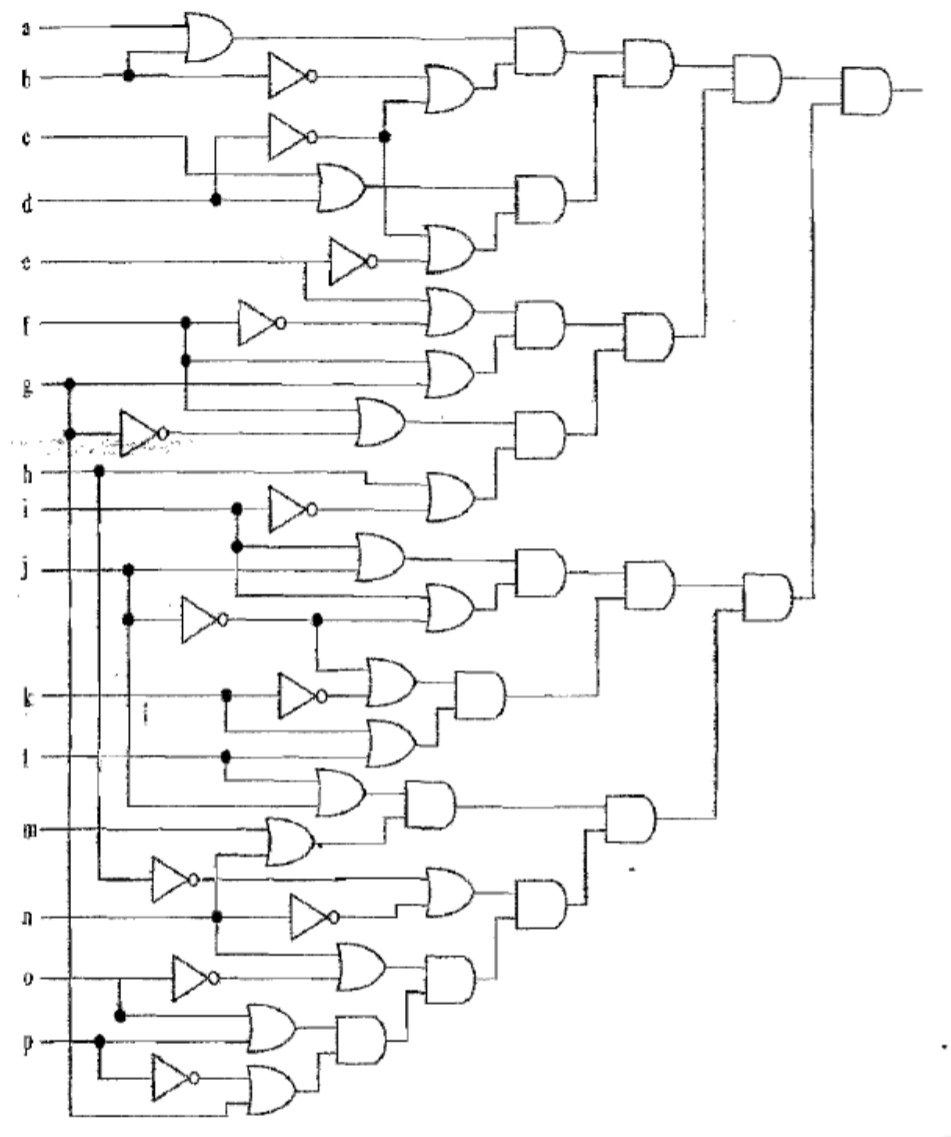
\includegraphics[width=0.65\textwidth]{circuit.png}
    \caption{Circuit with 16 inputs (labeled a-p)}
    \label{fig:circuit}
\end{figure}

\subsection{Algorithms and Libraries}
We use a simple brute force algorithm where we test each of the 65536 possible inputs to see if any outputs 1. When we find one, we print the combination and we update our solution count. When all the tasks are done we print the number of solutions. 

\medskip
\noindent
We parallelize the algorithm and check each of the 65536 combinations in parallel. The only dependency we need to be careful of is updating the solution counter and we use a reduction for this.

\medskip
\noindent
Libraries used:
\begin{itemize}
	\item \texttt{<omp.h>}
    \item \texttt{<math.h>}
    \item \texttt{<stdlib.h>}
    \item \texttt{<stdio.h>}
\end{itemize}

\subsection{Functions and Program Structure}
The program has 5 functions:
\begin{itemize}
    \item \texttt{main}
    \item \texttt{usage}
    \item \texttt{check\_circuit}
    \item \texttt{time\_parallel}
    \item \texttt{time\_serial}
\end{itemize}

\subsubsection{\texttt{main}}
Arguments: 
    \begin{itemize}
	    \item \texttt{int argc}: Number of command-line arguments.
        \item \texttt{char* argv[]}: Pointer array storing each command-line argument. 
    \end{itemize}
Returns: \texttt{0} indicating normal termination.

\medskip
\noindent
Description: 
\begin{itemize}
    \item Takes in 2 command-line arguments \texttt{print} and \texttt{reps} and checks them for valid range. Calls usage function if invalid.

    \item Declares variables and calls the parallel and serial functions to run and time each method.

    \item Prints the time taken by each method.
\end{itemize}

\subsubsection{\texttt{usage}}
Arguments: 
    \begin{itemize}
	    \item \texttt{char* prog\_name}: Character array containing the name of the program.
    \end{itemize}
Returns: void

\medskip
\noindent
Description: Prints a message explaining how to run the program.

\subsubsection{\texttt{check\_circuit}}
Arguments: 
    \begin{itemize}
	    \item \texttt{int id}: ID of the process calling the function.
	    \item \texttt{int z}: One of the 65536 possible inputs.
        \item \texttt{int print}: Contains a 0 or 1 to suppress or allow printing within the function. 
    \end{itemize}
Returns: \texttt{1} or \texttt{0} indicating a \texttt{true} or \texttt{false} output from the circuit.

\medskip
\noindent
Description: 
\begin{itemize}
    \item Takes in an integer \texttt{z} representing one of the possible inputs to the circuit. Extracts each bit of \texttt{z} and stores it in an array.

    \item Uses an if statement to represent the circuit and test its satisfiability.

    \item Prints the input combination if it satisfies the circuit as well as the process id that calls the function.
\end{itemize}

\subsubsection{\texttt{time\_parallel}}
Arguments: 
    \begin{itemize}
	    \item \texttt{int inputs}: Number of possible inputs (65536 in this case).
	    \item \texttt{int thread\_count}: Number of threads to parallelize the \texttt{for} loop.
	    \item \texttt{int reps}: Number of times to repeat the algorithm.
        \item \texttt{int print}: Contains a 0 or 1 to suppress or allow printing within the \texttt{check\_circuit} function.
    \end{itemize}
Returns: Time taken to run the algorithm averaged over \texttt{reps} times.

\medskip
\noindent
Description: 
\begin{itemize}
    \item Runs the algorithm to check the circuit satisfiability \texttt{reps} times. Keeps a track of how long each run takes.

    \item Evaluates the output for each of the 65536 inputs in parallel with \texttt{thread\_count} threads.

    \item Keeps a track of the number of inputs that satisfies the circuit and prints it out.
\end{itemize}

\subsubsection{\texttt{time\_serial}}
Arguments: 
    \begin{itemize}
	    \item \texttt{int inputs}: Number of possible inputs (65536 in this case).
	    \item \texttt{int reps}: Number of times to repeat the algorithm.
        \item \texttt{int print}: Contains a 0 or 1 to suppress or allow printing within the \texttt{check\_circuit} function.
    \end{itemize}
Returns: Time taken to run the algorithm averaged over \texttt{reps} times.

\medskip
\noindent
Description: 
\begin{itemize}
    \item Runs the algorithm to check the circuit satisfiability \texttt{reps} times. Keeps a track of how long each run takes.

    \item Evaluates the output for each of the 65536 inputs serially.

    \item Keeps a track of the number of inputs that satisfies the circuit and prints it out.
\end{itemize}

\subsection{Compilation and Usage}
Compilation: \texttt{make prog1}

\noindent
Usage: \texttt{./prog1 <print> <reps>}

\medskip
\noindent
Both programs can be compiled and linked at the same time using the command \texttt{make all}. To get rid of the executables in the folder, run the command \texttt{make clean}.

\medskip
\noindent
To use the program, we have a couple of command-line options to make it easier to test and experiment as we time our parallel and serial functions. 
\begin{itemize}
    \item The \texttt{print} variable expects an input of 0 or 1 corresponding to 'suppress printing' or 'allow printing' respectively.
    \item The \texttt{reps} variable is so that we can run both the serial and parallel algorithms multiple times and get a meaningful time comparison. Expects a value greater than or equal to 1.
\end{itemize}

\noindent
To run the program once with printing of every solution:

\texttt{./prog1 1 1}

\noindent
To time the program and suppress printing, bump up the number of repetitions and use 0 for the print variable:

\texttt{./prog1 0 1000}

\subsection{Testing and Verification}
To verify the program once we had our solution, we put our solution into Google and found that other people had published the same answer as us.
\begin{figure}[ht]
    \centering
    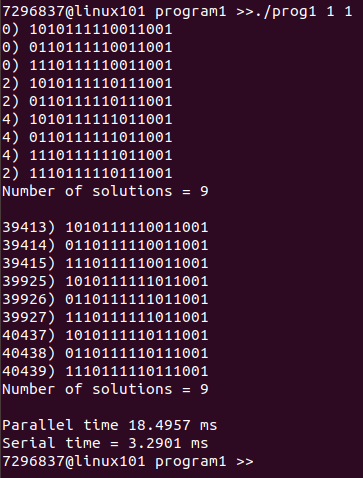
\includegraphics[width=0.45\textwidth]{verification.png}
    \caption{Solutions to the circuit}
    \label{fig:verification}
\end{figure}

\noindent
Once we verified that we had the right answer, we moved onto timing the two versions of the program, the parallel and serial. As you can see in figure \ref{fig:verification}, running the program just once doesn't really give us an accurate idea of how long each implementation takes. So, we built in a way to suppress the printing and increase the number of times the algorithm is run.

\begin{figure}[ht]
    \centering
    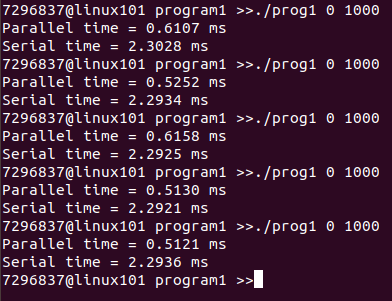
\includegraphics[width=0.45\textwidth]{prog1_timing.png}
    \caption{Comparing times for \texttt{prog1} with 1000 \texttt{reps}}
    \label{fig:prog1_timing}
\end{figure}

\subsubsection{Scheduling}
We tried using the OpenMP loop scheduler to see if we could better our performance. While the \texttt{schedule(static, 1)} showed a marginal improvement in performance, like we saw in class, \texttt{schedule(dynamic, 1)} does not do very well. This can be seen in figure \ref{fig:prog1_static_dynamic}. 

\begin{figure}[ht]
	\centering
    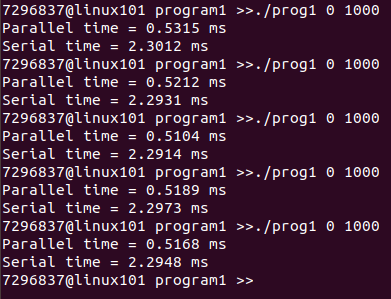
\includegraphics[width=0.45\textwidth]{prog1_timing_static.png}\quad
    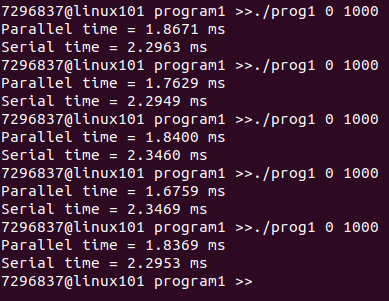
\includegraphics[width=0.45\textwidth]{prog1_timing_dynamic.png}\quad
    \caption{Comparison of the static and dynamic schedulers}
    \label{fig:prog1_static_dynamic}
\end{figure}

\noindent 
It should be noted that the dynamic scheduler does achieve a comparable performance to the static scheduler when the chunk size is increased.

\newpage

\section{Sieve of Eratosthenes}

\subsection{Introduction}
We are looking to find all the prime numbers up to an integer \texttt{n} using Eratosthenes' method. 

\begin{figure}[ht]
    \centering
    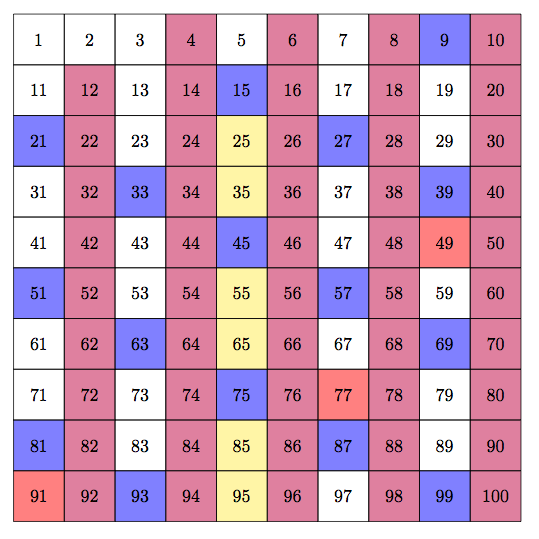
\includegraphics[width=0.55\textwidth]{sieve.png}
    \caption{Sieve of Eratosthenes up to 100}
    \label{fig:sieve}
\end{figure}

We would also like to parallelize the algorithm to improve our speed in finding all the primes less than or equal to \texttt{n}.

\subsection{Algorithms and Libraries}
The sieve of Eratosthenes algorithm is as follows:
\begin{enumerate}
    \item Create a list of consecutive integers from 2 through \texttt{n}: \texttt{(2, 3, 4, ..., n)}.
    
    \item Initially, let \texttt{p} equal 2, the first prime number.
    
    \item Starting from \texttt{p}, enumerate its multiples by counting to \texttt{sqrt(n)} in increments of \texttt{p}, and mark them in the list. These will be 2\texttt{p}, 3\texttt{p}, 4\texttt{p}, etc. (\texttt{p} itself should not be marked).
    
    \item Find the first number greater than \texttt{p} in the list that is not marked. If there was no such number, stop. Otherwise, let \texttt{p} now equal this new number (which is the next prime), and repeat from \texttt{step 3}.
\end{enumerate}

\medskip
\noindent
When we look at this algorithm, it is clear that \texttt{step 3} can be parallelized. We could also parallelize \texttt{step 4} but we might do extra work, finding multiples of a number that isn't prime. While this won't give us an incorrect answer, it might slow us down. We have opted to only parallelize \texttt{step 3} of the algorithm.

\medskip
\noindent
Libraries used: 
\begin{itemize}
	\item \texttt{<math.h>}
	\item \texttt{<omp.h>}
    \item \texttt{<stdlib.h>}
    \item \texttt{<stdio.h>}
\end{itemize}

\subsection{Functions and Program Structure}
The program has 6 functions:
\begin{itemize}
    \item \texttt{main}
    \item \texttt{usage}
    \item \texttt{time\_parallel}
    \item \texttt{time\_serial}
    \item \texttt{output}
    \item \texttt{output\_testing}
\end{itemize}

\subsubsection{\texttt{main}}
Arguments: 
    \begin{itemize}
	    \item \texttt{int argc}: Number of command-line arguments.
        \item \texttt{char* argv[]}: Pointer array storing each command-line argument. 
    \end{itemize}
Returns: \texttt{0} indicating normal termination.

\medskip
\noindent
Description: 
\begin{itemize}
    \item Takes in 3 command-line arguments \texttt{n}, \texttt{print}, and \texttt{reps} and checks them for valid range. Calls usage function if invalid.

    \item Declares variables and initializes the list tracking all the primes with 1s. 
    
    \item Calls the parallel and serial functions to run and time each method.

    \item Prints primes until \texttt{n} and the time taken by the parallel and serial methods.
\end{itemize}

\subsubsection{\texttt{usage}}
Arguments: 
    \begin{itemize}
	    \item \texttt{char* prog\_name}: Character array containing the name of the program.
    \end{itemize}
Returns: void

\medskip
\noindent
Description: Prints a message explaining how to run the program.

\subsubsection{\texttt{time\_parallel}}
Arguments: 
    \begin{itemize}
	    \item \texttt{int reps}: Number of times to repeat the algorithm.
	    
	    \item \texttt{unsigned long long n}: Used to calculate length of primes array.
	    
	    \item \texttt{unsigned long long* primes}: Pointer to array containing list of numbers to be 'sieved'.
    \end{itemize}
Returns: Time taken to run parallel portion of the algorithm averaged over \texttt{reps} times.

\medskip
\noindent
Description: 
\begin{itemize}
    \item Runs the sieve of Eratosthenes algorithm parallelizing \texttt{step 3} with \texttt{thread\_count} threads. Times how long this section of the algorithm takes.

    \item Runs the algorithm \texttt{reps} times to get an average of the running time.
\end{itemize}

\subsubsection{\texttt{time\_serial}}
Arguments: 
    \begin{itemize}
	    \item \texttt{int reps}: Number of times to repeat the algorithm.
	    
	    \item \texttt{unsigned long long n}: Used to calculate length of primes array.
	    
	    \item \texttt{unsigned long long* primes}: Pointer to array containing list of numbers to be 'sieved'.
    \end{itemize}
Returns: Time taken to run \texttt{step 3} of the algorithm averaged over \texttt{reps} times.

\medskip
\noindent
Description: 
\begin{itemize}
    \item Runs the sieve of Eratosthenes algorithm serially. Times how long \texttt{step 3} of the algorithm takes.

    \item Runs the algorithm \texttt{reps} times to get an average of the running time.
\end{itemize}

\subsubsection{\texttt{output}}
Arguments: 
    \begin{itemize}
	    \item \texttt{unsigned long long n}: Used to calculate length of primes array.
	    
	    \item \texttt{unsigned long long* primes}: Pointer to array of prime numbers.
    \end{itemize}
Returns: void

\medskip
\noindent
Description: 
\begin{itemize}
    \item Calculates padding value to print with correct formatting.

    \item Prints all the primes from 2 to \texttt{n} with 10 on each row.
\end{itemize}

\subsubsection{\texttt{output\_testing}}
Arguments: 
    \begin{itemize}
	    \item \texttt{unsigned long long n}: Used to calculate length of primes array.
	    
	    \item \texttt{unsigned long long* primes}: Pointer to array of prime numbers.
    \end{itemize}
Returns: void

\medskip
\noindent
Description: 
Prints all the primes from 2 to \texttt{n} matching the output format of the test file from \url{http://www.mathematical.com/primes0to1000k.html} so that we can run a diff on the two files.

\subsection{Compilation and Usage}
Compilation: \texttt{make prog2}

\noindent
Usage: \texttt{./prog2 <n> <print> <reps>}

\medskip
\noindent
Both programs can be compiled and linked at the same time using the command \texttt{make all}. To get rid of the executables in the folder, run the command \texttt{make clean}.

\medskip
\noindent
To use the program, we have a couple of command-line options to make it easier to test and experiment as we time our parallel and serial functions. 
\begin{itemize}
    \item \texttt{n} expects a value greater than or equal to 2. The program finds all the primes less than or equal to \texttt{n}.
    
    \item The \texttt{print} variable expects an input of 0 or 1 corresponding to 'suppress printing' or 'allow printing' respectively.
    
    \item The \texttt{reps} variable is so that we can run both the serial and parallel algorithms multiple times and get a meaningful time comparison. Expects a value greater than or equal to 1.
\end{itemize}

\noindent
To run the program and print all primes less than 1 million:

\texttt{./prog2 1000000 1 1}

\noindent
To time the program and suppress printing, bump up the number of repetitions and use 0 for the print variable:

\texttt{./prog2 1000000 0 100}

\subsection{Testing and Verification}
To verify the program once we had our solution, we looked for a list of primes online that didn't have a very challenging output formatting. This was so that we could adapt our print function with a few tweaks and run a diff on the two files.

\begin{figure}[ht]
    \centering
    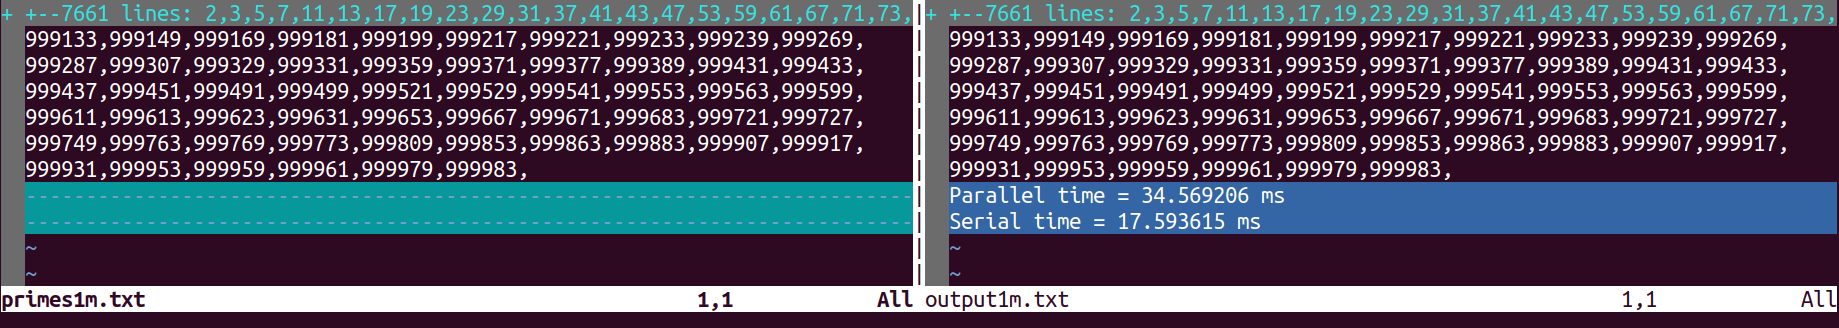
\includegraphics[width=\textwidth]{vimdiff.png}
    \caption{Running \texttt{vimdiff} on \texttt{primes1m.txt} and \texttt{output1m.txt}}
    \label{fig:vimdiff}
\end{figure}

\medskip
\noindent
We ended up picking the list on \url{http://www.mathematical.com/primes0to1000k.html}, creating one small file and one large file. The test files can be found in the testfiles/ directory. Files beginning with "primes*" are created from the website, "output*" are files created by our program. Running a diff on the pairs of files, the only difference should be the timing output statements at the end of the file. Figure \ref{fig:vimdiff} shows an example of the diff between a pair of files to verify our list of primes.

\medskip
\noindent
Once we verified that we had the right answer, we moved onto timing the two versions of the program, the parallel and serial. Like in \texttt{prog1}, running the program just once doesn't give us an accurate idea of how long each implementation takes. So again, we increase the number of times we run the algorithm and average the time.

\begin{figure}[ht]
    \centering
    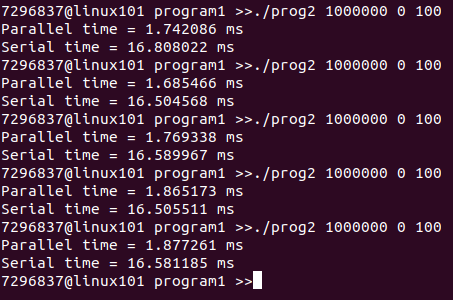
\includegraphics[width=0.45\textwidth]{prog2_timing.png}
    \caption{Comparing times for \texttt{prog2} with 100 \texttt{reps}}
    \label{fig:prog2_timing}
\end{figure}

\subsubsection{Scheduling}
We tried using the OpenMP loop scheduler to see if we could better our performance. As expected, \texttt{schedule(dynamic, 1)} again gives very poor results - worse than the serial solution this time. Surprisingly, for this algorithm, even \texttt{schedule(static, 1)} shows a worse performance than if we do not specify the loop scheduler (Figure \ref{fig:prog2_static_dynamic}). 

\begin{figure}[ht]
	\centering
    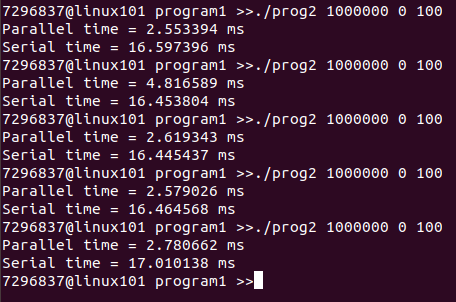
\includegraphics[width=0.45\textwidth]{prog2_timing_static.png}\quad
    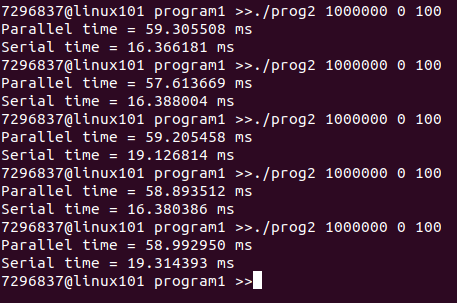
\includegraphics[width=0.45\textwidth]{prog2_timing_dynamic.png}\quad
    \caption{Comparison of the static and dynamic schedulers}
    \label{fig:prog2_static_dynamic}
\end{figure}

\noindent 
Again, it should be noted that by playing around with the chunk size parameter does achieve a better performance than sticking with the default value of 1.

\section{Files Submitted}
\begin{itemize}
    \item \texttt{prog1.pdf}
    \item \texttt{Makefile}
    \item \texttt{prog1.c}
    \item \texttt{prog2.c}
    \item \texttt{testfiles/}
    \item \texttt{latex/}
\end{itemize}

\end{document}
